\chapter[Implementering af software]{Software}

% Note om hvad der skal stå i dette afsnit her.


\section{Oversigt over softwaren}

% Her skriver vi hvordan softwaren er struktureret - se figuren nedenfor.

Softwaren er struktureret som vist i
figur\vref{fig:software-oversigt}. Dataføderen leverer data til den
del af softwaren, der behandler HPGL. Dataen kommer fra et
SD-kort. HPGL-behandleren sender instruktioner videre til den del af
motorkontrollen, der afvikles når der er tid. Denne del sætter
instruktioner i kø til realtidsdelen.

Realtidsdelen af motorkontrollen behandler de instruktioner, den anden
del af motorkontrollen har sat i kø og styrer stepmotorer m.m. efter
disse instruktioner. Realtidsdelen af motorkontrollen har ansvar for,
at hastigheden af tegnehovedet kan styres præcist.


\begin{figure}[htbp]
  \centering
  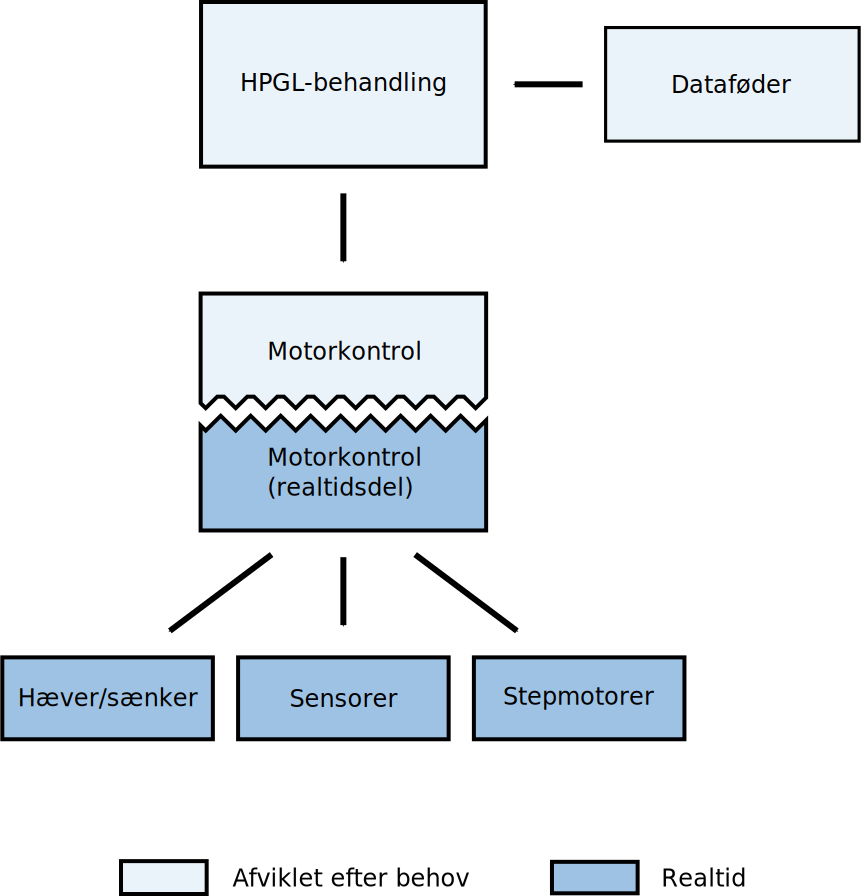
\includegraphics[width=.75\textwidth]{../brugere/kjaergaard/software-oversigt}
  \caption{Oversigt over softwaren. De lyseblå dele afvikles når der
    er tid til det. Når det er tid til at afvikle de mørkeblå områder,
    afbrydes afviklingen af de lyseblå.}
  \label{fig:software-oversigt}
\end{figure}


\section[Dataføder (med SPI og SD-/MMC-kort)]{Dataføder}

% Hvordan virker dataføderen (herunder buffer, spi og sd/mmc)?

Dataføderen leverer data til HPGL-motoren og håndterer de
underliggende moduler, der indeholder data.

Dataføderens skal
\begin{itemize} \firmlist
\item levere data til HPGL-motoren og sørge for at denne ikke løber
  tør for data\fixme{bliv enig om terminologi}
\item stille et uniformt API\footnote{Application Programming
    Interface, programmeringsbrugerflade; betegnelse for struktur og
    navngivning for funktioner, variable, strukturer, klasser
    etc. brugt til programudvikling.}\fixme{brug evt. wikis
    formulering af api} til rådighed uafhængig af underliggende modul,
  således at det overliggende modul er uafhængig af det modul, der
  indeholder data - se figur\vref{fig:datafeeder-uniform-api}
\item håndtere fejl for underliggende moduler
\end{itemize}

\mnote{
  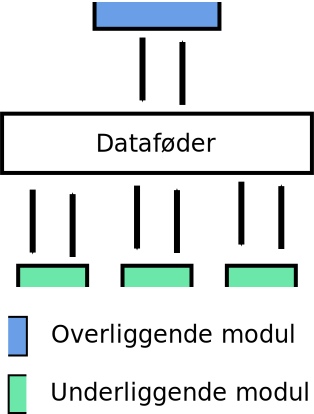
\includegraphics[width=\marginparwidth]{../brugere/kjaergaard/datafoeder-uniform-api}
  \captionof{figure}{Data\-føderen skal stille et uniformt API til
    rådighed.}
  \label{fig:datafeeder-uniform-api}
}

En oversigt over funktionsfordelingen\fixme{andet ordvalg} i
dataføreren\fixme{andet ordvalg} kan ses i
figur\vref{fig:software-spi-sd-oversigt}.

\begin{figure}[htbp]
  \centering
  \includegraphics[width=\textwidth]{../brugere/kjaergaard/datafeeder-oversigt}
  \caption{Diagram over funktionsfordeling i dataføderen.}
  \label{fig:software-spi-sd-oversigt}
\end{figure}

Kommunikationen med SD-kortet foregår gennem SPI'en.\fixme{afsnit skal
  skrives færdig}. En eksempel på en forespørgsel med tilhørende svar
kan ses i figur\vref{fig:software-spi-sd-handling}.

\begin{figure}[htbp]
  \centering
  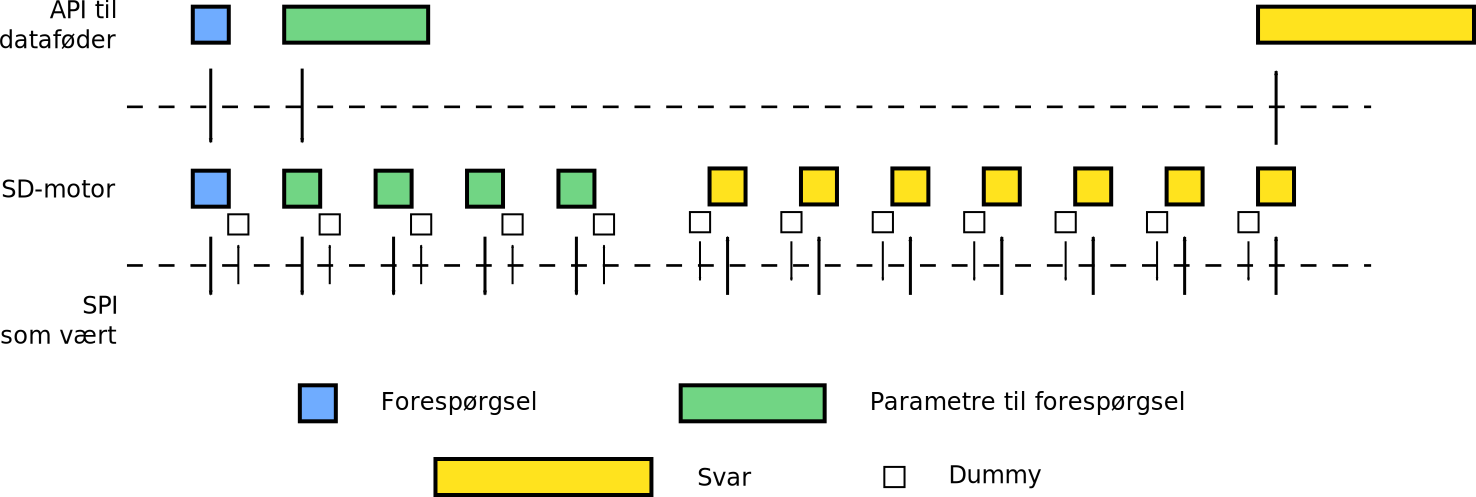
\includegraphics[width=\textwidth]{../brugere/kjaergaard/datafeeder-handling}
  \caption{Handlingdiagram ved kommunikation med SD-kortet.}
  \label{fig:software-spi-sd-handling}
\end{figure}


\section{HPGL-behandleren}

% Hvordan virker den del, der fortolker og behandler HPGL?


\subsection{Identifikation af instruktioner og parametre}

% Her skriver vi hvordan vi identificerer instruktioner og parametre i
% datastrømmen



\subsection{Matematik -- Cirkel}
\mnote{
  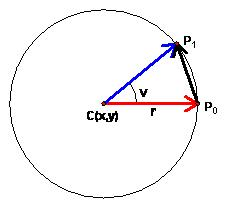
\includegraphics[width=\marginparwidth]{./img/Cirkel}
  \captionof{figure}{Cirkel}
  \label{fig:cirkel-tegning}
}
Vi kender cirklens radius, kordevinklen samt startkoordinater. Det første koordinat kan derfor let findes:
\begin{align*}
P_0(x, y)=(r, 0)
\end{align*}

Næste koordinat ligger i en vinkel v, som svarer til kordevinklen c. Ved brug af cosinus og sinus samt radius kan vi bestemme det næste koordinat:
\begin{align*}
P_1(x, y)&=(\cos(v)\times r, \sin(v)\times r)\Rightarrow \\
P_1(x, y)&=(\cos(c)\times r, \sin(c)\times r)
\end{align*}
 
Denne formel kan omskrives, så den gælder et vilkårligt punkt på cirkelperiferien:
\begin{align}
P_n(x, y)=(\cos(n\times c)\times r, \sin(n\times c)\times r)
\end{align}

Vi betragter nu en cirkel med en radius på 5cm og en kordevinkel på $3\degree$. Første koordinat er således:
\begin{align*}
P_0(x, y)=(\cos(0\times 3\degree , \sin(0\times 3\degree)\times 5)=(5, 0)
\end{align*}

Vi ser, at dette passer i overensstemmelse med første udsagn. Vha. ovenstående formel kan vi blot lægge en til n hver gang funktionen er udført. Dette skal den blive ved med indtil vinkel overskrider $360\degree$.


Der opstår dog et problem, hvis vinklen ikke går op i $360\degree$, såsom vinklen $7\degree$. $51\times 7\degree = 357\degree \Rightarrow rest = 3\degree$. Overskrider vinklen de $360\degree$, har vi to muligheder:
\begin{itemize} \firmlist
\item Funktionen afsluttes uden at slutte cirklen
\item Funktionen ændres, så optegningen fortsætter til udgangspunktet $P_0$
\end{itemize}
Det skal også nævnes, at HPGL tegner uanset om pennen er oppe eller nede, hvilket betyder, at vi skal bruge en funktion til at hæve og sænke pennen. Pennen starter i cirklens centrum. Vi skal derfor sikre os, at pennen er hævet før den går til første punkt  . Herefter bruger vi den generelle funktion til at bestemme x,y-koordinaterne. Efter hver udført funktion lægges en ekstra kordevinkel til vinklen indtil vinklen v er større eller lig $360\degree$. Herefter hæves pennen og flyttes tilbage til cirklens centrum. Afviklingsdiagrammet viser denne proces (se \vref{fig:hpgl-cirkel-afvikling}).

\begin{figure}[htbp]
  \centering
  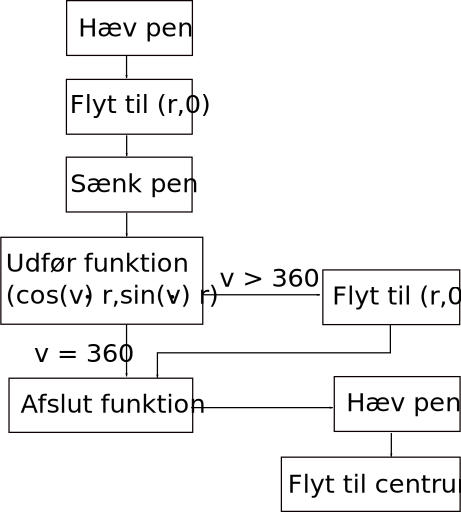
\includegraphics[width=0.5\textwidth]{./img/Afviklingsdiagram_Cirkel}
  \caption{Afviklingsdiagram for cirkelplot}
  \label{fig:hpgl-cirkel-afvikling}
\end{figure}

\section[Motorkontrol (med buffer)]{Motorkontrol}

% Hvordan er motorkontrollen implementeret? Beskriv implementeringen
% kort.


\section{Stepmotorstyring}

% Hvordan styres stepmotorerne? Superkort. Hvordan ser softwaren der
% styrer dem ud?


\section{Sensorer og løfter/sænker}


\section{HPGL -- Hewlett-Packard Graphics Language}

% Hvordan implementerer vi HPGL? Hvilke afvigelser tillader vi os at
% tage fra den dokumentation, vi har fundet?


%%% Local Variables: 
%%% mode: latex
%%% TeX-master: "../master"
%%% End: 